
\documentclass[12pt, letterpaper, twoside]{article}
\usepackage[utf8]{inputenc}
\usepackage{graphicx}
\usepackage{subfigure}
\usepackage{adjustbox}
\usepackage{caption}
%\usepackage{subcaption}
\usepackage{amsmath} 
\bibliographystyle{elsarticle-num}

\title{Pion Multiplicity Analysis}
\author{Justin Estee}
\date{June 2019}
\graphicspath{ {Images/} }


\begin{document}

 
\begin{titlepage}
\maketitle
\end{titlepage}
 
 \section{Introduction}
 The purpose of this document is to outline (in detail) the method used to get the total pion multiplicity and the multiplicity spectra.
 
 In our data we have several corrections we must account for to get the multiplicity spectra and the total pion multiplicity per event. This includes getting the total number of events measured, correcting for the efficiency, and correcting for the total solid angle not covered. 
 
 \section{Center of Mass Transformation}
 After rotating the beam event by the beam angles provided by Jon, our system is now rotated event-by-event to align with the TPC z-axis. Now using the K.E. of the beam calculated from Jon (BigRIPS analysis), we can transform to the COM system by performing a Lorentz transformation to the COM by applying $-\beta$ to the Lorentz transform matrices in the ROOT class TLorentzVector. The calculation for $\beta$ is given in Eq. \ref{eq:beta} where $E_{Beam}=~K.E._{Beam} + M_{Beam}$ and $p_{Beam}$ is the momentum of the beam in the Lab frame. 
 
 \begin{equation}
 \beta = \frac{\vert p_{Beam} \vert}{E_{Beam} + M_{Target}}
 \label{eq:beta}
 \end{equation}
 
 \section{Cuts on the Data}
The data has been cut in the good region of efficiency in the lab frame ($\theta_{Lab}$ $<$ 70 \&\& ($\phi$ $<$ 30 \&\& $\phi$ $>$ 330) $||$ 150 $<$ $\phi$ $<$ 210) and then transformed to the Center of Mass (COM) system as shown in Fig. \ref{fig:data}.

Several other quality cuts were made:
\begin{itemize}
\item ${}^{132}$Sn beam PID cut
\item On target vertex cut
\item Distance-to-vertex $<$ 20mm
\item Number-of-clusters $>$ 15
\item Multiplicity $>$ 50
\item No Gating Grid fast close events
\end{itemize} 

These are the typical data cuts we take to get clean PID. All of these cuts are reasonable quality cuts and do not place too much of a bias on the data. 
 

 
 \begin{figure*}
\begin{adjustbox}{max width=1.2\linewidth,center}
\centering
\subfigure[Lab frame]{\label{fig:a}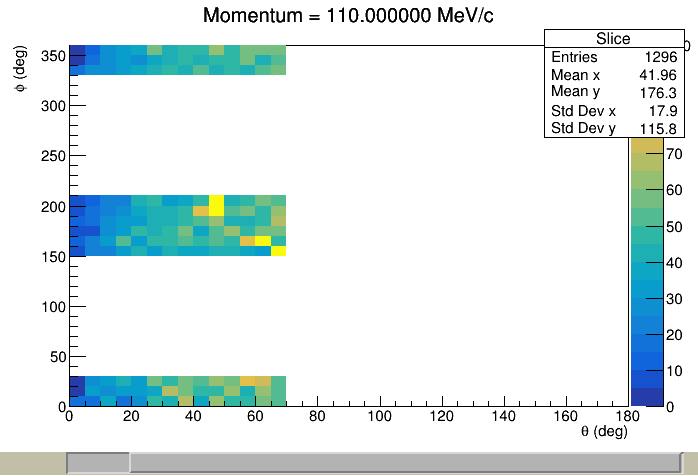
\includegraphics[width=0.7\textwidth]{dataLab.png}}%
\subfigure[Transformed to Center of Mass]{\label{fig:b}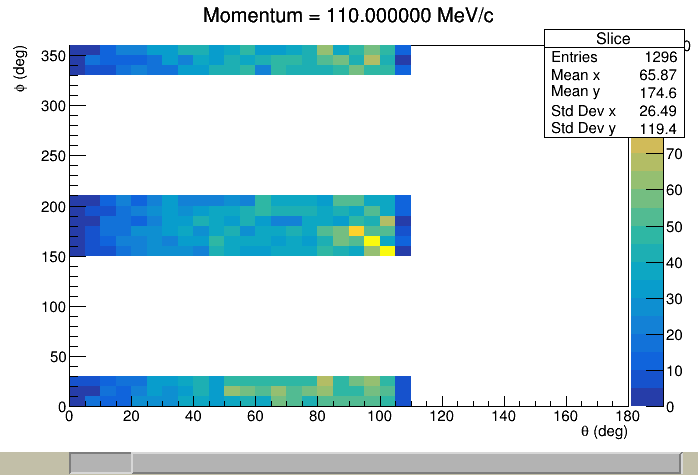
\includegraphics[width=0.7\textwidth]{dataCOM.png}}%
\end{adjustbox}
\label{fig:data}
 \caption{$\pi^+$ data within cut, $\theta_{Lab}$ $<$ 70 \&\& ($\phi$ $<$ 30 \&\& $\phi$ $>$ 330) $||$ 150 $<$ $\phi$ $<$ 210 }
 \label{fig:data}
\end{figure*}
 
 \section{Efficiency Correction}
 \subsection{Embedding MC Tracks}
 We are embedding simulated MC tracks (which take into account most of the TPC detector physics) into real data events. This way we can incorporate effects such as saturation, track multiplicity, detector bias, detector acceptance, software inefficiency, and other effects that are otherwise too hard to directly simulate. A measured known MC track is digitized and embedded and the whole event is reconstructed. The embedded hits are tagged and tracked through the full software reconstruction. We embedded into real data events that are in the vertex cut and the beam PID cut condition (i.e. ${}^{132}$Sn beam PID cut from Jon's BigRIPS analysis).
 
  After the event is reconstructed there are three possible outcomes, there are no embedded tracks reconstructed, there is one embedded track found, or there are several embedded tracks found. The first two cases are very straightforward (either the embedded track is found or not), in the latter case is the case of track splitting. Several effects in the TPC (both physical and in software) which can cause a track to split. All reconstructed embedded tracks are saved in an array which can be studied in detail.
 
 For the purpose of this paper we are not interested in track splitting and we need to make a choice on which track measured corresponds to input MC track, without biasing the results. It would be easiest to just match the known MC input momentum with the final track momentum, but this would bias the results to be more like the MC input momentum. Since we are interested in studying what happens to the momentum the track with the smallest distance-to-vertex is taken as the track which is most likely resembles the input MC track. This makes logical sense since all the MC track must originate from the TPC vertex. 
 
 Once we have the reconstructed track, combined with the information for the MC input track, we can approach the situation of calculating efficiency. 
 
 \subsection{Method to Calculate Efficiency}
 The efficiency calculation is done bin-by-bin. A uniform distribution of pions in momentum, $p$, and angles $\theta$, and $\phi$ is input into the embedding analysis. A database of the input and output tracks from the embedding is made. The efficiency is calculated simply by subdividing the phase space ($p$,$\theta$,$\phi$) into several bins. 
 Then calculating the efficiency is simply looping over the database from the embedding results and calculating the ratio of tracks detected divided by tracks input for each bin, as in Eq. \ref{eq:eff_cal}. Where $N(p,\theta,\phi)_{detected}$ is the total number of tracks detected and $N(p,\theta,\phi)_{total}$ represents the total number of tracks input. 
 
 A track which is ``$detected$" is classified as a track which was reconstructed in the embedding process and survives the cuts placed on the data set. This could mean any cut, $dE/dx$, distance to vertex, multiplicity, or cluster number. The total number of tracks is the total number of tracks within the multiplicity cut and the phase space region of interest.
   
 \begin{equation} 
 \label{eq:eff_cal}
 \epsilon_{(p,\theta,\phi)} = \frac{N(p,\theta,\phi)_{detected}}{N(p,\theta,\phi)_{total}}
 \end{equation}  
  
  
\subsection{Efficiency Corrected Spectra}
 
 
 \section{Correcting for the Integrated Solid Angle}
 Since the TPC is a fixed target, "box`` shaped detector, the angular coverage does not cover the full solid angle of $4\pi$. Because of the quality angle cuts placed in Fig~\ref{fig:data}, only around 20\% of $4\pi$ (in the COM) is covered. Furthermore, since the angular coverage also depends slightly on the momentum of the pion, we must also correct for the solid angle covered by the TPC for a given momentum. 
 
 Using a uniform distribution in $\theta$,$\phi$, and momentum $p$, as an input to the MC embedding procedure, we can determine the angular coverage of the TPC by putting the same cuts in the Lab frame (as Fig.~\ref{fig:data}) then transforming to the COM system to see the angular coverage of the TPC.
 
 Since the MC embedding has no information of the beam, remember we are just evaluating efficiency in different lab angles, we assume a value of $\beta = -.364$ for transforming the MC embedded tracks to the COM frame. The momentum acceptance calculated by Jon shows that the $\beta$ distribution is sharply peaked, with little variation, around this value. 
 
For this analysis I have not put in the angle rotation for the MC track coverage calculation. Seen in Fig.~\ref{fig:cutcov} is the coverage in the COM system for the given Lab frame cuts in Fig.~\ref{fig:data}. The coverage depends on the momentum of the system but for these cuts the $\pi{-}$ and $\pi^+$ coverages are almost the same for a given momentum. 


\begin{figure*}
\begin{adjustbox}{max width=1.2\linewidth,center}
\centering
\subfigure[70 MeV/c $\pi^{+}$]{\label{fig:a}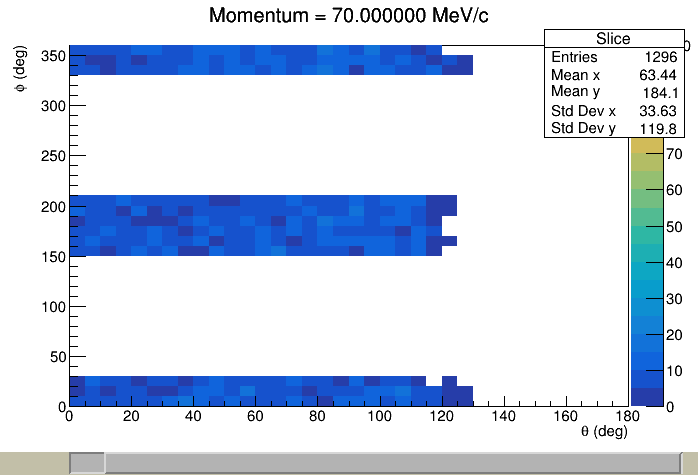
\includegraphics[width=0.35\textwidth]{70Mev}}%
\subfigure[310 MeV/c $\pi^{+}$]{\label{fig:b}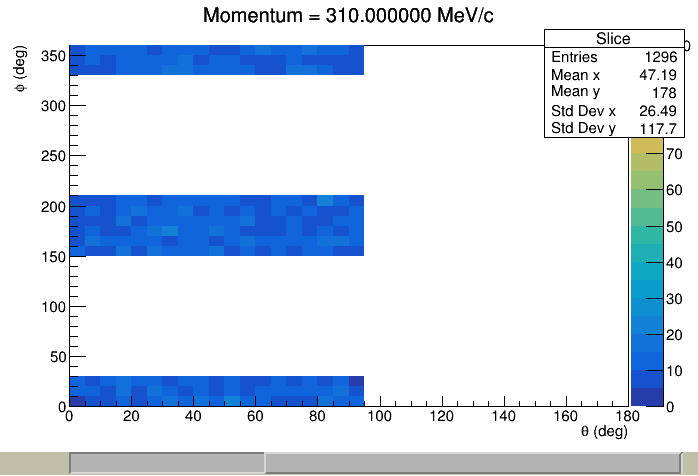
\includegraphics[width=0.35\textwidth]{310MeV}}%
\subfigure[410 MeV/c $\pi^{+}$]{\label{fig:c}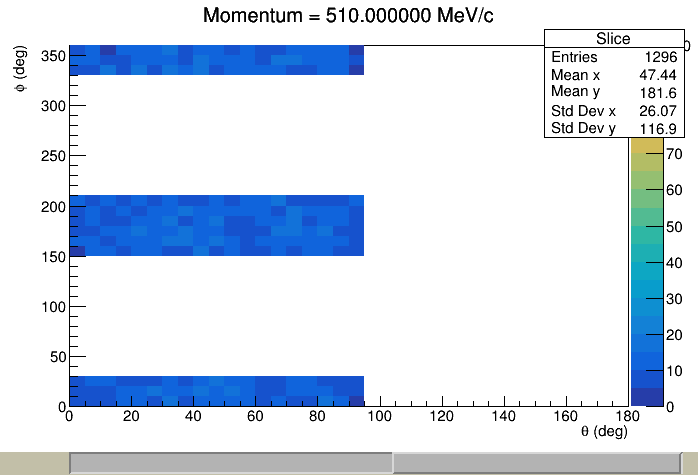
\includegraphics[width=0.35\textwidth]{510MeV}}%
\end{adjustbox}
\label{fig:cutcov}

\medskip

\begin{adjustbox}{max width=1.2\linewidth,center}
\centering
\subfigure[70 MeV/c $\pi^{-}$]{\label{fig:d}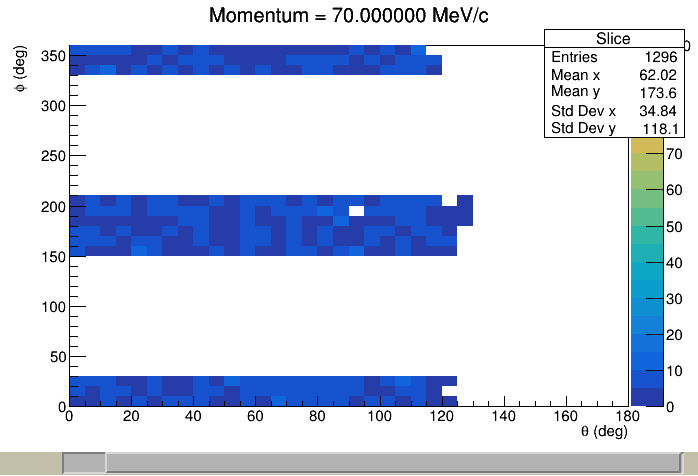
\includegraphics[width=0.35\textwidth]{pim70MeV}}%
\subfigure[310 MeV/c $\pi^{-}$]{\label{fig:e}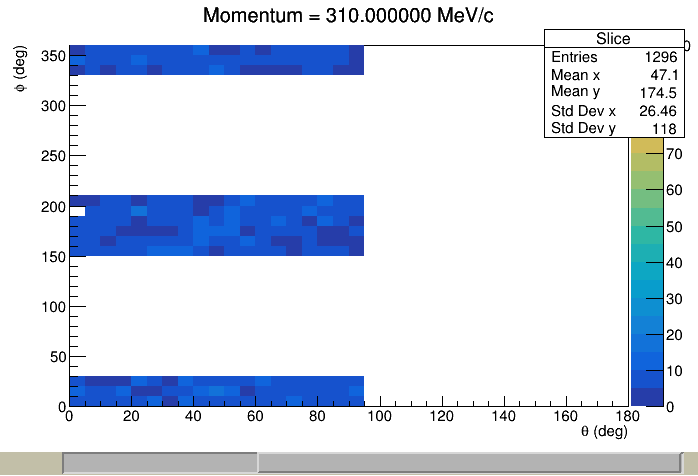
\includegraphics[width=0.35\textwidth]{pim310MeV}}%
\subfigure[410 MeV/c $\pi^{-}$]{\label{fig:f}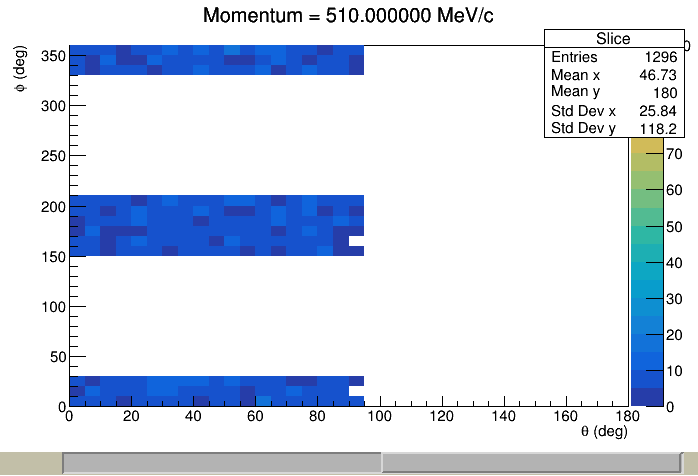
\includegraphics[width=0.35\textwidth]{pim510MeV}}%
\end{adjustbox}
\caption{$\theta_{Lab}$ $<$ 70 \&\& ($\phi$ $<$ 30 \&\& $\phi$ $>$ 330) $||$ 150 $<$ $\phi$ $<$ 210 cut coverage in COM coordinates. From MC embedding of uniform distribution in $\phi$, $\theta$, and $p$}
\end{figure*}
 
 We now can calculate the solid angle covered in the COM system by summing the total solid angle covered by each bin as given in Eq.~\ref{eq:solid}, where $\theta_H$ and $\theta_L$ are the high and low limits of the bin in $\theta$, and $\phi_H$ and $\phi_L$ are the high and low limits in $\phi$ respectively. 
 
 \begin{equation}
 \Omega = \sum (\cos(\theta_L) - \cos(\theta_H))(\phi_H - \phi_L)
 \label{eq:solid}
 \end{equation}
 
 This is done for each momentum bin, which is assigned a total angular coverage of $\Omega_p$, for each momentum value, $p$. It is a good assumption that in the COM system the $\pi$ distribution is nearly isotropic. Correcting for the areas of the solid angle coverage we correct the counts in each momentum bin, $N_p$, by ${4\pi/\Omega_p}$, since this is the inverse of the fraction of space we measure in the TPC. 
 
 \subsection{Solid Angle and Efficiency Corrected Spectra}


 
 \section{Calculation of Impact Parameter}
 I refer to Jon for details of how he gets the impact parameter from cross section measurements. What he and Genie has provided us is with a tool to calculate the impact parameter estimate from the multiplicity distribution. For a multiplicity cut of $>$ 50, this corresponds to an impact parameter range of 0 $<$ b $<$ 3.5 [fm] with an average of 2.4 [fm]. This is important for later where we will calculate the total number of participants for these numbers. The range in $b$ will help us to estimate our error bar on the total number of participants. 
 
 \section{Calculation of Number of Participants $A_{part}$}
 The total number of particles in the participant region of the collision is calculated using the Glauber model where each nuclei is given a random isotropic distribution in $\phi$ and $\theta$, where a random number between 0 and 1 is chosen, $rand[0,1]$, and input into Eq.~\ref{eq:randphi} and Eq.~\ref{eq:randtheta}, to generate random isotropic points in spherical angles. The radius is randomly sampled from $4\pi r^{2}\rho(r)$, where the absolute normalization is not important. $\rho(r)$ is given in Eq~\ref{eq:radial} where $R=5.45$ and $a=.4835$ for ${}^{132}$Sn and $R=5.38$ and $a=.4835$ for the ${}^{124}$Sn, as plotted in Fig.~\ref{fig:radial}.
 
 \begin{equation}
 \phi = rand[0,1] * 2\pi
 \label{eq:randphi}
 \end{equation}
 
 \begin{equation}
  \theta = (2*rand[0,1] - 1)
  \label{eq:randtheta}
 \end{equation}
 
 \begin{equation}
 \rho(r) = \rho_{o} \frac{1}{1+ exp(\frac{r-R}{a})}
 \label{eq:radial}
 \end{equation}
 
 
  \begin{figure*}
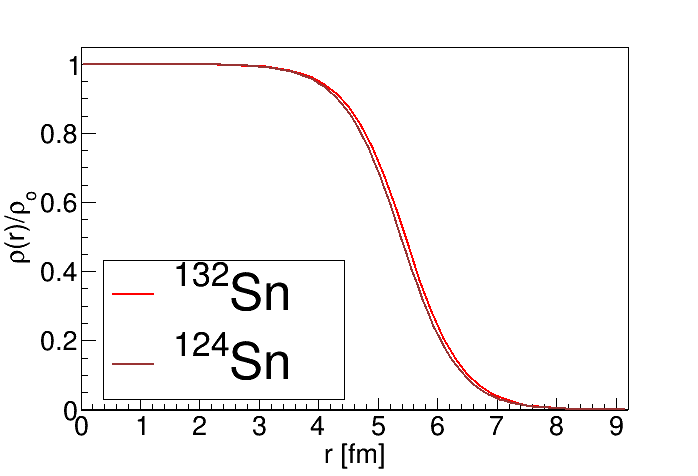
\includegraphics[width=\textwidth]{density.png}
 \caption{Radial nucleon density.}
 \label{fig:radial}
\end{figure*}

 The nuclei are initialized to be separated by a distance of $b$, center to center, as given by the impact parameter you choose. The nuclei are then collided by small time steps and at each step the distance to each pair of nucleons, $d$, is calculated. If ,$d < \sqrt{ \frac{ \sigma_{nn} }{\pi}}$, then the nucleons are said to have collided (and are therefore are "participants``), where $\sigma_{nn}$ is the nucleon-nucleon free cross section, which is a constant 33$mb$ (or 3.3 $fm^2$), for a range of incident energies we cover in our experiments. Thus the distance in which nucleons are said to collide is about $d < 1fm$. I then measure the total number of particles which collided to get the number of participants, $A_{part}$.
 
 Since this is a MC method it is averaged over several MC trials to arrive at the average number for $A_{part}$. Table~\ref{tb:apart} shows a list of the $A_{part}$ for various impact parameters. The total number of MC Glauber model collisions was 1000 to reduce the statistical error bar in the calculation. 

\begin{table}[!htb]
\begin{center}
 \begin{tabular}{||c c||}
 \hline
 ${}^{132}$Sn + ${}^{124}$Sn \\ [0.5ex] 
 \hline\hline
 b [fm] & $A_{part}$ \\ [0.5ex]
 \hline\hline
 0 &  255.6 \\
 \hline
 1 & 254.0 \\ 
 \hline
 2.4 & 244.2\\
 \hline
 3.45 & 232.0\\
 \hline
 4 & 220.6 \\
 \hline
 5 & 197.4 \\ 
 \hline
 6 & 158.0 \\ [1ex] 
 \hline
\end{tabular}
\end{center}
\caption{$A_{part}$ for a given impact parameter b in the Glauber model}
\label{tb:apart}
\end{table}

Shown in Fig.~\ref{fig:coll} is the Glauber collision (projected onto the x-z plane) for the initial, middle, and final stages of the collision. 

\begin{figure}[!hbt]

\begin{adjustbox}{max width=\linewidth,center}
\centering
\subfigure[Initial stage]{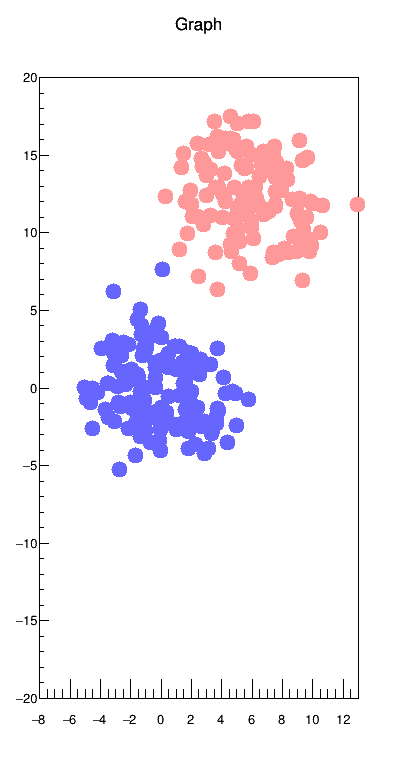
\includegraphics[width=0.35\textwidth]{step_0.png}}%
\subfigure[Middle stage]{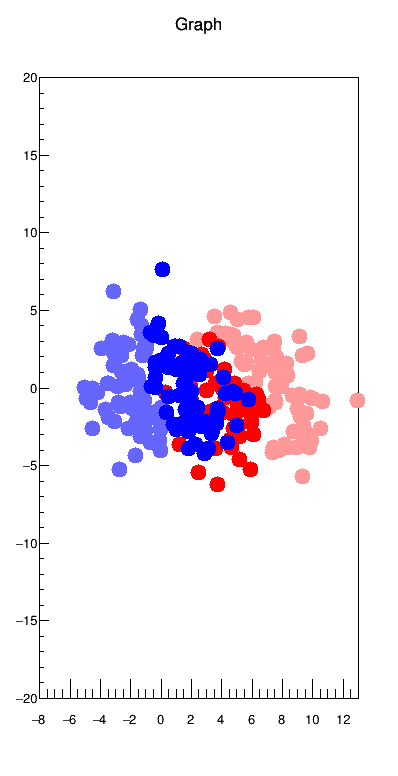
\includegraphics[width=0.35\textwidth]{step_50.png}}%
\subfigure[Final stage]{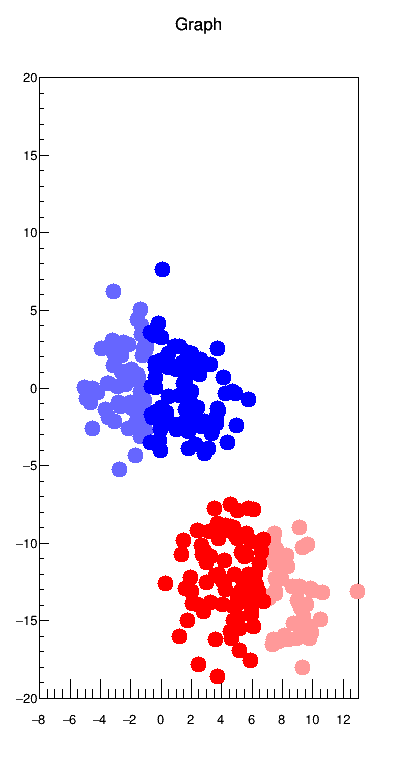
\includegraphics[width=0.35\textwidth]{step_99.png}}%
\end{adjustbox}
\caption{Glauber model in initial, middle, and final stage of the collision. Light colors denote spectators and vivid colors participants. Blue denotes target and red denotes projectile.}
\label{fig:coll}

\end{figure}

\clearpage

\section{Pion Multiplicity}
In \cite{fopi}, the total pion multiplicity is defined as $M(\pi)=1.5(M(\pi^-)+M(\pi^+))$. Integrating the pion efficiency (and solid angle corrected) pion spectra in FIGURE, we can get the total pion multiplicities for ${}^{132}$Sn. 

\begin{table}[!htb]
\begin{center}
 \begin{tabular}{||c c c c c||}
 \hline
  & ${}^{132}$Sn + ${}^{124}$Sn & ${}^{108}$Sn + ${}^{112}$Sn & ${}^{124}$Sn + ${}^{112}$Sn & ${}^{112}$Sn + ${}^{124}$Sn\\ [0.5ex] 
 \hline\hline
  $M(\pi^-)$ & 2  & 2 & 2 & \\ [0.5ex]
 \hline\hline
 $M(\pi^+)$ &  255.6  &  2 & 2 & \\
 \hline
\end{tabular}
\end{center}
\caption{Pion multiplicities.}
\label{tb:pionmult}
\end{table}

\section{Comparing With FOPI Data}



\subsection{Correction for $A_{part}$ Effect on $M(\pi)$}


\begin{figure}[!hbt]

\begin{adjustbox}{max width=\linewidth,center}
\centering
\subfigure[With $A_{part}$ correction]{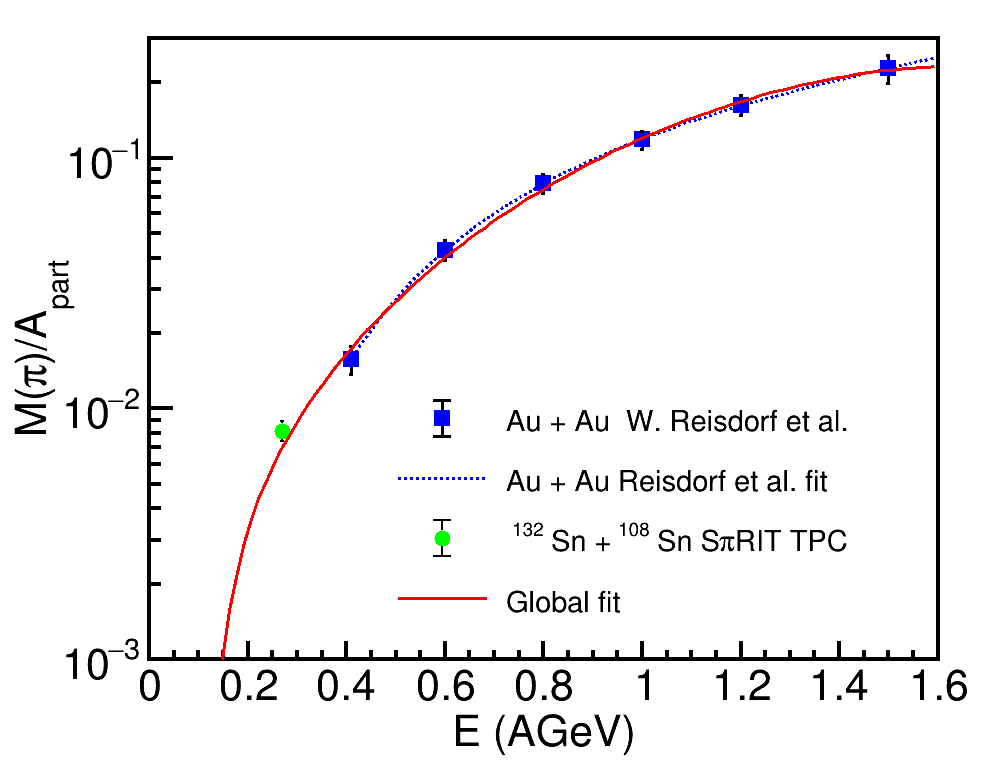
\includegraphics[width=0.5\textwidth]{multiplicitypion.png}}%
\subfigure[No correction]{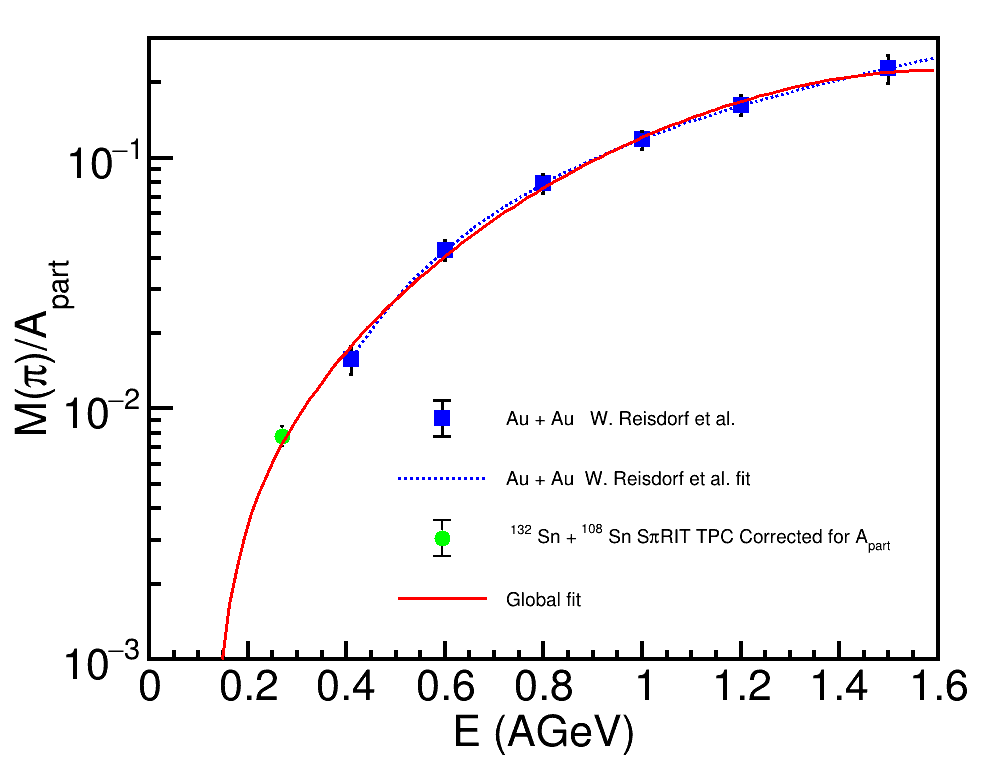
\includegraphics[width=0.5\textwidth]{multiplicitypion_scaled.png}}%
\end{adjustbox}
\caption{Pion multiplicity before and after correction, compared with FOPI data.}
\label{fig:mult}

\end{figure}

\subsection{N/Z Effect for $\pi^-/\pi^+$}
It is well known that the $\pi^-/\pi^+ \propto (n/z)^2$, at low energies. Because of this dependence we need to correct the ${}^{197}$Au + ${}^{197}$Au FOPI data (which has $N/Z= 1.49$), and extrapolate the  $\pi^-/\pi^+$ to $N/Z=1.56$, for the ${}^{132}$Sn~+~${}^{124}$Sn system. Plotted in Fig.~\ref{fig:nzdepend} is the N/Z dependence published in the FOPI data set \cite{fopi}. The measured data points are given in the blue circles. The paper cites a linear fit was applied to the data which I have plotted at the black dotted line. The paper also says a linear extrapolation was performed to extrapolate to $N/Z=1.56$. One can see the blue "X`` are the points which they calculate, which matches the linear extrapolation. For .8 and 1 A GeV the linear extrapolation seems reasonable but for .4 A GeV we know the dependence should be $(n/z)^2$, as is clear from the trend of the data. I extrapolated the $N/Z=1.56$ for .4 AGeV which is shown as the green point in Fig.~\ref{fig:nzdepend}, and also in .8 and 1 AGeV. 


\begin{figure}[!hbt]
\centering
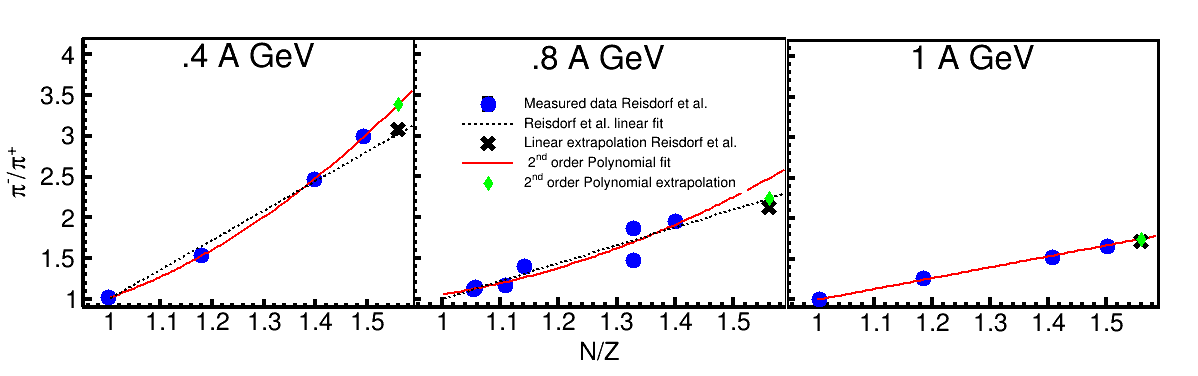
\includegraphics[width=\textwidth]{NZDependence.png}
\caption{$\pi^-/\pi^+$ N/Z dependence }
\label{fig:nzdepend}
\end{figure}
 
 In Fig.~\ref{fig:pionratio}, the total pion ratio extended to $N/Z=1.56$ is plotted in the blue and red points, the blue points representing the pion ratio from the FOPI experiment (with their fit), and the red points representing the error in extrapolating .4 AGeV which I described above. The ${}^{132}$Sn+${}^{124}$Sn is plotted in green. We can see a good agreement (considering the red points are not data but extrapolated data), also considering the correct extrapolation at .4 AGeV is made. Error bars to come. 
 
\begin{figure}[!hbt]
\centering
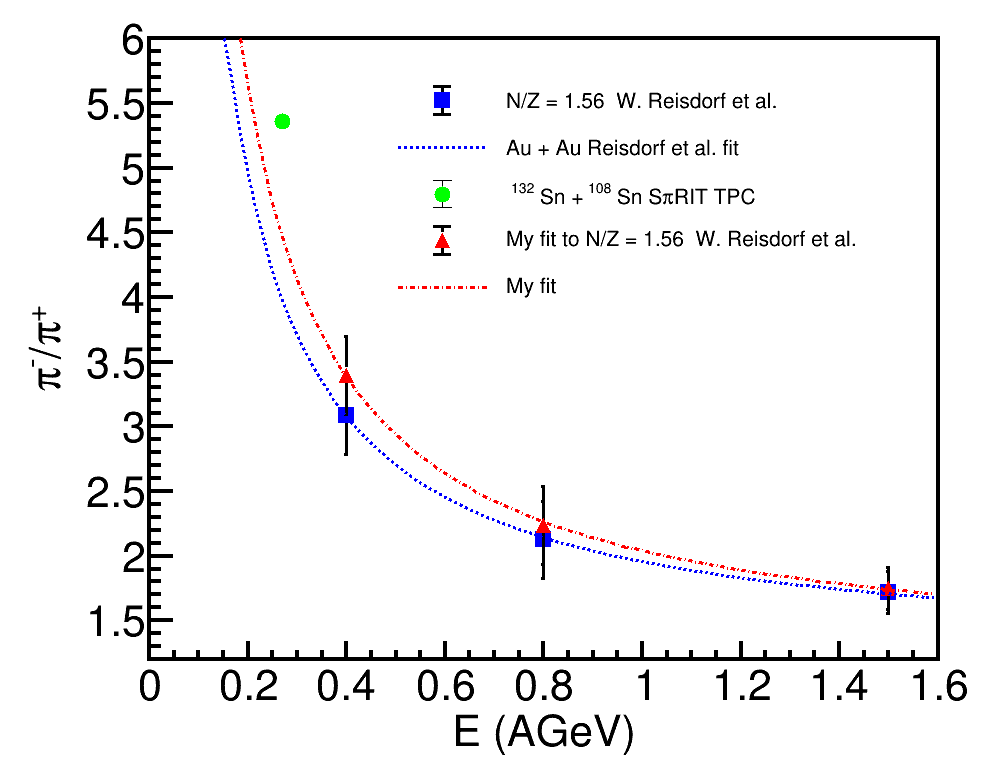
\includegraphics[width=\textwidth]{pionratio.png}
\caption{$\pi^-/\pi^+$ for $N/Z=1.56$}
\label{fig:pionratio}
\end{figure}
 
 
 
 
 
 
\newpage
\bibliography{mybibfile}

 
 
\end{document}

